\documentclass[11pt,letterpaper]{article}

% Packages
\usepackage[utf8]{inputenc}
\usepackage[margin=1in]{geometry}
\usepackage{graphicx}
\usepackage{hyperref}
\usepackage{xcolor}
\usepackage{fancyhdr}
\usepackage{titlesec}
\usepackage{tocloft}
\usepackage{tabularx}
\usepackage{longtable}
\usepackage{booktabs}
\usepackage{enumitem}
\usepackage[expansion=false]{microtype}
\usepackage{float}
\usepackage{tikz}
\usetikzlibrary{shapes.geometric, arrows.meta, positioning, shadows, backgrounds, calc}

% Define brand colors
\definecolor{blockdblue}{RGB}{0,102,204}
\definecolor{blockdgray}{RGB}{64,64,64}
\definecolor{accentgreen}{RGB}{16,185,129}
\definecolor{accentorange}{RGB}{251,146,60}
\definecolor{lightgray}{RGB}{243,244,246}

% Hyperref setup
\hypersetup{
    colorlinks=true,
    linkcolor=blockdblue,
    filecolor=magenta,
    urlcolor=blockdblue,
    pdftitle={Blockd - Investor Presentation},
    pdfauthor={Blockd Inc.},
}

% TikZ styles for diagrams - FIXED FOR NO OVERLAP
\tikzset{
    box/.style={rectangle, rounded corners, minimum width=2.8cm, minimum height=0.9cm,
                text centered, text width=2.5cm, draw=blockdblue, fill=blockdblue!10,
                drop shadow, font=\small},
    highlight/.style={rectangle, rounded corners, minimum width=2.8cm, minimum height=0.9cm,
                      text centered, text width=2.5cm, draw=accentgreen, fill=accentgreen!20,
                      drop shadow, line width=1.2pt, font=\small},
    arrow/.style={thick,-{Stealth[length=3mm]},blockdblue}
}

% Header and footer
\pagestyle{fancy}
\fancyhf{}
\rhead{\textcolor{blockdblue}{Blockd Investor Presentation}}
\lhead{\textcolor{blockdgray}{Confidential}}
\cfoot{\thepage}

% Section formatting
\titleformat{\section}
  {\color{blockdblue}\normalfont\Large\bfseries}
  {\thesection}{1em}{}
\titleformat{\subsection}
  {\color{blockdgray}\normalfont\large\bfseries}
  {\thesubsection}{1em}{}

% Title page
\title{
    \Huge\textbf{\textcolor{blockdblue}{Blockd}}\\
    \vspace{0.5cm}
    \Large Revolutionizing Remote Interview Integrity\\
    \vspace{0.5cm}
    \large AI-Powered Security Platform for Technical Hiring\\
    \vspace{1.5cm}
}
\author{
    \textbf{Blockd Inc.}\\
    \vspace{0.3cm}
    Investor Presentation\\
    \vspace{0.3cm}
    \textcolor{blockdgray}{Confidential \& Proprietary}
}
\date{November 2025\\Version 2.0}

\begin{document}

\maketitle
\thispagestyle{empty}
\newpage

% Confidentiality Notice
\thispagestyle{empty}
\vspace*{\fill}
\begin{center}
\fbox{\parbox{0.9\textwidth}{
\textbf{CONFIDENTIALITY NOTICE}

This document contains confidential and proprietary information belonging to Blockd Inc. This information is being shared solely for the purpose of evaluating a potential investment opportunity and may not be reproduced, distributed, or disclosed to any third party without the express written consent of Blockd Inc.

By accepting this document, the recipient agrees to maintain its confidentiality and return or destroy all copies upon request.

© 2025 Blockd Inc. All Rights Reserved.
}}
\end{center}
\vspace*{\fill}
\newpage

% Table of Contents
\tableofcontents
\newpage

%----------------------------------------------------------------------------------------
% EXECUTIVE SUMMARY
%----------------------------------------------------------------------------------------

\section{Executive Summary}

\subsection{The Opportunity}

The global technical hiring market is experiencing unprecedented challenges:

\begin{itemize}[noitemsep]
    \item \textbf{\$650+ billion} global recruitment and staffing industry (2025)\cite{qxglobal2025}
    \item \textbf{67\%} of hiring managers now use video interviews, up from 22\% pre-pandemic\cite{withe2024}
    \item \textbf{55\%} of companies report concerns about interview authenticity\cite{shrm2024}
    \item \textbf{\$15,000 - \$25,000} average cost per bad technical hire\cite{apollotechnical2025}
    \item \textbf{76\%} of developers use AI tools like ChatGPT and GitHub Copilot\cite{stackoverflow2024}
\end{itemize}

\textbf{Blockd} addresses this critical gap with the industry's first comprehensive AI-powered interview security platform, combining advanced machine learning, computer vision, and behavioral analysis to ensure interview integrity at scale.

\subsection{Our Solution}

Blockd is an enterprise-grade platform that provides:

\begin{enumerate}
    \item \textbf{AI-Powered Cheating Detection}: Proprietary multi-model analysis detects AI-generated answers with industry-leading accuracy
    \item \textbf{Real-time Security Monitoring}: Native browser-level security prevents screen recording, VM usage, and process manipulation
    \item \textbf{Behavioral Analysis}: Eye tracking and response timing analytics identify suspicious patterns
    \item \textbf{Comprehensive Reporting}: Automated risk scoring and detailed analytics for hiring decisions
\end{enumerate}

\subsection{Market Traction}

\begin{table}[H]
\centering
\begin{tabularx}{\textwidth}{lX}
\toprule
\textbf{Metric} & \textbf{Status} \\
\midrule
Platform Status & Production-ready, fully developed \\
Technology & 91,000+ lines of production code, 674+ files \\
Scalability & Designed for 1,000+ concurrent sessions \\
Testing & 68+ automated test scenarios \\
Infrastructure & Cloud-native, auto-scaling architecture \\
Security & Enterprise-grade encryption, GDPR compliant \\
\bottomrule
\end{tabularx}
\end{table}

\subsection{Investment Highlights}

\begin{itemize}[noitemsep]
    \item \textbf{Large Addressable Market}: \$3.3B+ technical recruitment software TAM\cite{coherent2024}
    \item \textbf{First-mover Advantage}: Comprehensive AI detection in interview security
    \item \textbf{High Margins}: SaaS model with 80-85\% gross margins
    \item \textbf{Scalable Technology}: Cloud-native architecture built for global deployment
    \item \textbf{Enterprise Ready}: Production-ready platform with Fortune 500-grade infrastructure
    \item \textbf{Defensible IP}: Proprietary AI detection algorithms and behavioral analysis models
\end{itemize}

%----------------------------------------------------------------------------------------
% MARKET OPPORTUNITY
%----------------------------------------------------------------------------------------

\section{Market Opportunity}

\subsection{Market Size \& Growth}

\begin{figure}[H]
\centering
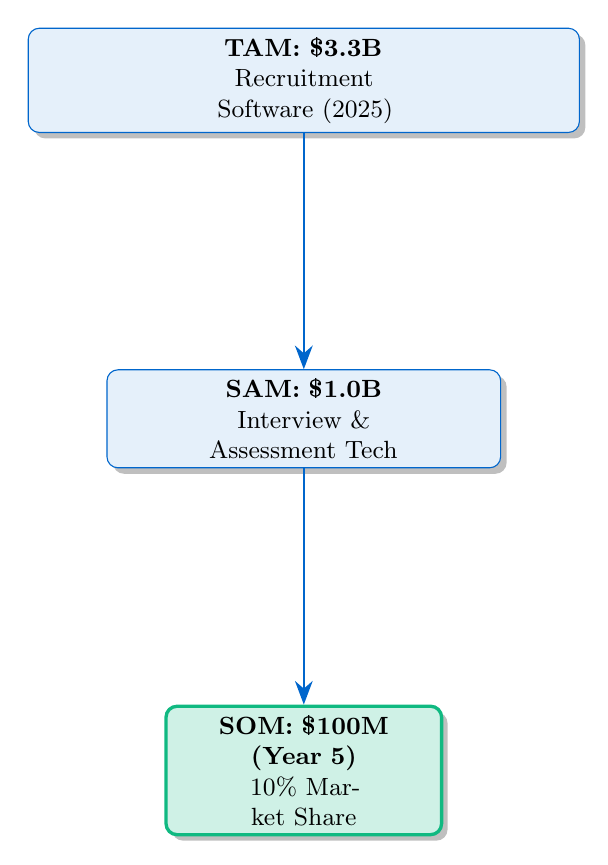
\begin{tikzpicture}[node distance=3cm]
    % TAM
    \node[box, minimum width=7cm, minimum height=1.2cm] (tam)
        {\textbf{TAM: \$3.3B} \\ Recruitment Software (2025)};

    % SAM
    \node[box, minimum width=5cm, minimum height=1.2cm, below=of tam] (sam)
        {\textbf{SAM: \$1.0B} \\ Interview \& Assessment Tech};

    % SOM
    \node[highlight, minimum width=3.5cm, minimum height=1.2cm, below=of sam] (som)
        {\textbf{SOM: \$100M (Year 5)} \\ 10\% Market Share};

    % Arrows
    \draw[arrow] (tam) -- (sam);
    \draw[arrow] (sam) -- (som);
\end{tikzpicture}
\caption{Market Segmentation \& Opportunity (Based on 2025 market data\cite{coherent2024,mordor2025})}
\end{figure}

\subsection{Market Drivers}

\begin{enumerate}
    \item \textbf{Remote Work Acceleration}
    \begin{itemize}
        \item 67\% of hiring managers now use video interviews\cite{withe2024}
        \item Permanent shift to hybrid/remote hiring models
        \item 93\% of employers plan to continue remote interviews\cite{adaface2024}
    \end{itemize}

    \item \textbf{AI Tool Proliferation}
    \begin{itemize}
        \item 76\% of developers use AI tools in development\cite{stackoverflow2024}
        \item 82\% specifically use ChatGPT; 68\% use GitHub Copilot\cite{stackoverflow2024}
        \item 60\% of graduates admit to using AI during interviews\cite{handshake2025}
    \end{itemize}

    \item \textbf{Interview Integrity Crisis}
    \begin{itemize}
        \item 70\%+ of job seekers admit to dishonesty during hiring\cite{resumetemplates2024}
        \item 55\% of hiring managers concerned about authenticity\cite{shrm2024}
        \item 37\% of cheaters used ChatGPT when prohibited\cite{resumetemplates2024}
    \end{itemize}

    \item \textbf{Cost of Bad Hires}
    \begin{itemize}
        \item \$15,000-\$25,000 average cost per bad hire\cite{apollotechnical2025}
        \item Can reach 75-150\% of salary for technical roles\cite{careerbuilder2024}
        \item 74\% of employers admit to hiring wrong candidates\cite{businesscom2024}
    \end{itemize}
\end{enumerate}

\subsection{Target Segments}

\begin{table}[H]
\centering
\small
\begin{tabularx}{\textwidth}{lXl}
\toprule
\textbf{Segment} & \textbf{Characteristics} & \textbf{Priority} \\
\midrule
Tech Companies & 500+ developers, high hiring volume, remote-first & Primary \\
Consulting Firms & Technical screening, high turnover, global teams & Primary \\
Financial Services & Regulatory requirements, security-critical roles & Secondary \\
Healthcare Tech & HIPAA compliance, specialized technical roles & Secondary \\
Government & Security clearances, stringent verification & Tertiary \\
\bottomrule
\end{tabularx}
\end{table}

%----------------------------------------------------------------------------------------
% PRODUCT OVERVIEW
%----------------------------------------------------------------------------------------

\section{Product Overview}

\subsection{Platform Architecture}

\begin{figure}[H]
\centering
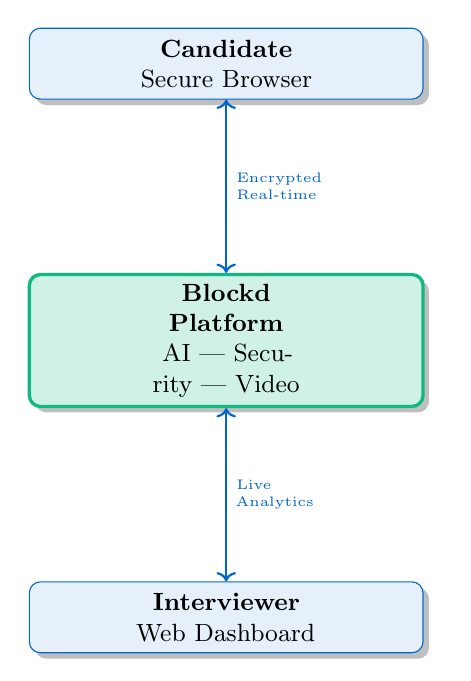
\begin{tikzpicture}[node distance=2.2cm]
    % Candidate Layer
    \node[box, minimum width=5cm] (candidate) {\textbf{Candidate} \\ Secure Browser};

    % Cloud Platform
    \node[highlight, minimum width=5cm, below=of candidate] (platform)
        {\textbf{Blockd Platform} \\ AI | Security | Video};

    % Interviewer Layer
    \node[box, minimum width=5cm, below=of platform] (interviewer)
        {\textbf{Interviewer} \\ Web Dashboard};

    % Arrows with labels
    \draw[arrow, <->] (candidate) -- node[right, font=\tiny, text width=2.5cm, align=left]
        {Encrypted \\ Real-time} (platform);
    \draw[arrow, <->] (platform) -- node[right, font=\tiny, text width=2.5cm, align=left]
        {Live \\ Analytics} (interviewer);
\end{tikzpicture}
\caption{Blockd Three-Tier Architecture}
\end{figure}

\subsection{Key Differentiators}

\begin{table}[H]
\centering
\small
\begin{tabularx}{\textwidth}{lXX}
\toprule
\textbf{Feature} & \textbf{Blockd} & \textbf{Alternatives} \\
\midrule
AI Detection & Multi-model analysis & Manual review only \\
Security Level & Native browser, unbypassable & Extensions (easily disabled) \\
Behavioral Analysis & Eye tracking + timing + patterns & Basic webcam \\
Real-time Alerts & Instant during interview & Post-interview only \\
Scalability & 1,000+ sessions & 10-50 sessions \\
Integration & API-first, SSO, HRIS & Standalone \\
\bottomrule
\end{tabularx}
\end{table}

%----------------------------------------------------------------------------------------
% CORE FEATURES
%----------------------------------------------------------------------------------------

\section{Core Features \& Benefits}

\subsection{1. AI-Powered Answer Detection}

\textbf{The Problem:} With 76\% of developers using AI tools\cite{stackoverflow2024}, candidates can generate perfect answers instantly.

\textbf{Our Solution:} Proprietary multi-model analysis compares answers against multiple AI engines.

\begin{figure}[H]
\centering
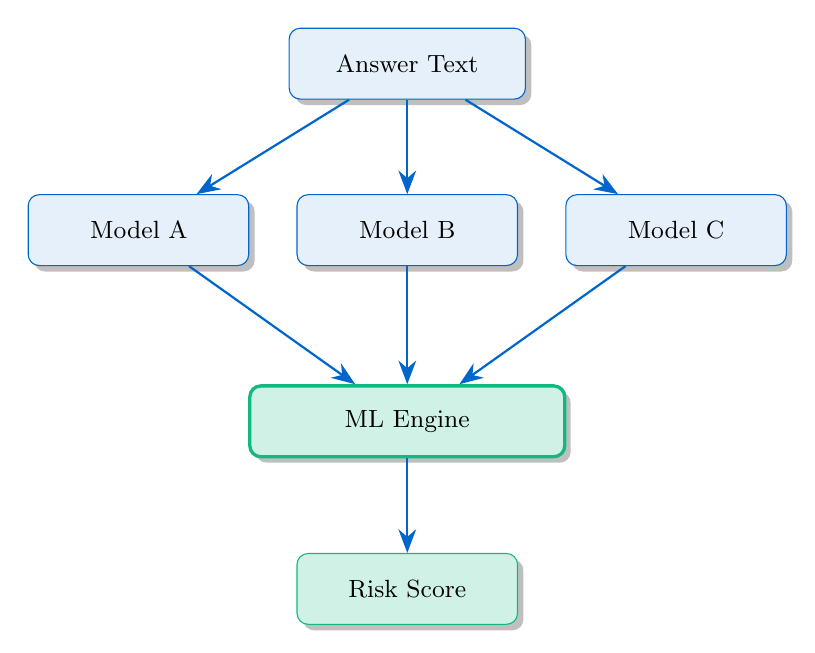
\begin{tikzpicture}[node distance=1.5cm]
    % Input
    \node[box, minimum width=3cm] (input) {Answer Text};

    % Analysis
    \node[box, below left=1.2cm and 0.5cm of input] (m1) {Model A};
    \node[box, below=1.2cm of input] (m2) {Model B};
    \node[box, below right=1.2cm and 0.5cm of input] (m3) {Model C};

    % Engine
    \node[highlight, below=1.5cm of m2, minimum width=4cm] (ml) {ML Engine};

    % Output
    \node[box, below=1.2cm of ml, fill=accentgreen!20, draw=accentgreen] (out) {Risk Score};

    % Arrows
    \draw[arrow] (input) -- (m1);
    \draw[arrow] (input) -- (m2);
    \draw[arrow] (input) -- (m3);
    \draw[arrow] (m1) -- (ml);
    \draw[arrow] (m2) -- (ml);
    \draw[arrow] (m3) -- (ml);
    \draw[arrow] (ml) -- (out);
\end{tikzpicture}
\caption{AI Detection Workflow}
\end{figure}

\textbf{Benefits:}
\begin{itemize}[noitemsep]
    \item Industry-leading detection accuracy
    \item <5 second analysis time
    \item Confidence scoring for hiring decisions
    \item Reduces false hires significantly
\end{itemize}

\subsection{2. Native Browser Security}

\textbf{The Problem:} Browser extensions are easily detected and disabled by tech-savvy candidates.

\textbf{Our Solution:} Custom secure browser with embedded, unbypassable monitoring.

\textbf{Detection Capabilities:}
\begin{itemize}[noitemsep]
    \item ✓ Screen recording software (OBS, Camtasia, etc.)
    \item ✓ Virtual machines (VMware, VirtualBox, Parallels)
    \item ✓ Remote access tools (TeamViewer, AnyDesk)
    \item ✓ Window focus changes
    \item ✓ Clipboard monitoring
    \item ✓ Process enumeration
\end{itemize}

\subsection{3. Behavioral Analytics}

\textbf{The Problem:} Candidates reading from second monitors or receiving off-camera help.

\textbf{Our Solution:} Computer vision eye tracking at 30 FPS with ML-powered pattern analysis.

\textbf{Benefits:}
\begin{itemize}[noitemsep]
    \item Detects off-screen reading (second monitor)
    \item Identifies unnatural response patterns
    \item Real-time gaze heatmaps
    \item Pattern recognition for suspicious behavior
\end{itemize}

\subsection{4. Comprehensive Reporting}

\begin{table}[H]
\centering
\begin{tabularx}{\textwidth}{lXX}
\toprule
\textbf{Report Type} & \textbf{Contents} & \textbf{Use Case} \\
\midrule
Real-time & Live events, gaze, AI alerts & During interview \\
Summary & Risk score, incidents, timestamps & Post-interview \\
Executive & Trends, recommendations & Management \\
Audit Trail & Complete logs, compliance & Regulatory \\
\bottomrule
\end{tabularx}
\end{table}

%----------------------------------------------------------------------------------------
% USE CASES
%----------------------------------------------------------------------------------------

\section{Use Cases \& ROI}

\subsection{High-Volume Tech Recruiting}

\textbf{Customer Profile:} Tech companies hiring 100+ developers annually

\textbf{ROI Example:}
\begin{itemize}[noitemsep]
    \item Company hiring 200 developers/year
    \item Without Blockd: 10 bad hires × \$20,000 = \textbf{\$200,000 loss}
    \item With Blockd: 3 bad hires × \$20,000 = \textbf{\$60,000 loss}
    \item Annual Savings: \$140,000
    \item Platform Cost: \$30,000/year
    \item \textbf{Net ROI: 367\%}
\end{itemize}

\subsection{Consulting \& Staffing Firms}

\textbf{Value Proposition:}
\begin{itemize}[noitemsep]
    \item Quality assurance for contractor placements
    \item Audit trail for client confidence
    \item Scalable to 1,000+ monthly interviews
    \item Reduces client churn from bad placements
\end{itemize}

\subsection{Enterprise Security-Critical Roles}

\textbf{Use Case:} Financial services, healthcare, government contractors

\textbf{Benefits:}
\begin{itemize}[noitemsep]
    \item Complete audit trail with video evidence
    \item Regulatory compliance documentation
    \item Security clearance verification support
    \item Multi-region data residency
\end{itemize}

%----------------------------------------------------------------------------------------
% COMPETITIVE LANDSCAPE
%----------------------------------------------------------------------------------------

\section{Competitive Landscape}

\subsection{Market Positioning}

\begin{figure}[H]
\centering
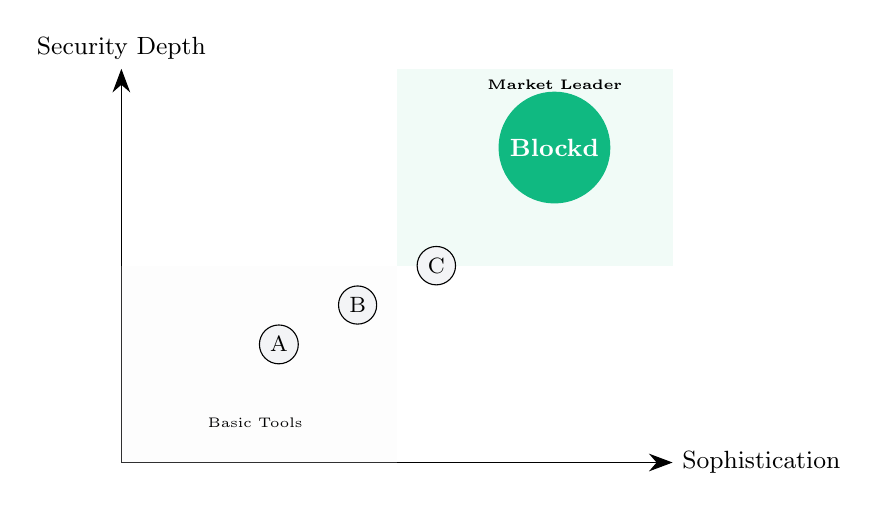
\begin{tikzpicture}[scale=1.0]
    % Axes
    \draw[-{Stealth[length=3mm]}] (0,0) -- (7,0) node[right, font=\small] {Sophistication};
    \draw[-{Stealth[length=3mm]}] (0,0) -- (0,5) node[above, font=\small] {Security Depth};

    % Quadrant shading
    \fill[lightgray, opacity=0.2] (0,0) rectangle (3.5,2.5);
    \fill[accentgreen!15, opacity=0.4] (3.5,2.5) rectangle (7,5);

    % Competitors
    \node[circle, draw, fill=lightgray, inner sep=2pt, font=\footnotesize] at (2,1.5) {A};
    \node[circle, draw, fill=lightgray, inner sep=2pt, font=\footnotesize] at (3,2) {B};
    \node[circle, draw, fill=lightgray, inner sep=2pt, font=\footnotesize] at (4,2.5) {C};

    % Blockd
    \node[circle, draw=accentgreen, fill=accentgreen, text=white, inner sep=3pt,
          font=\small\bfseries] at (5.5,4) {Blockd};

    % Labels
    \node[font=\tiny, text width=2cm, align=center] at (1.7,0.5) {Basic Tools};
    \node[font=\tiny, text width=2cm, align=center] at (5.5,4.8) {\textbf{Market Leader}};
\end{tikzpicture}
\caption{Competitive Positioning Matrix}
\end{figure}

\subsection{Competitive Advantages}

\begin{table}[H]
\centering
\footnotesize
\begin{tabularx}{\textwidth}{lX}
\toprule
\textbf{Advantage} & \textbf{Description} \\
\midrule
Technology Depth & Only solution combining AI + native security + behavioral analytics \\
Bypass Prevention & Native browser eliminates circumvention (extensions easily disabled) \\
Real-time & Instant alerts during interviews vs. post-interview only \\
Scalability & 1,000+ sessions vs. competitors' 10-50 \\
Enterprise Features & SSO, API, HRIS, multi-region \\
Proprietary IP & Custom ML models, detection heuristics \\
\bottomrule
\end{tabularx}
\end{table}

%----------------------------------------------------------------------------------------
% BUSINESS MODEL
%----------------------------------------------------------------------------------------

\section{Business Model \& Go-to-Market}

\subsection{Revenue Model}

\textbf{SaaS Subscription Pricing} (Annual Contracts)

\begin{table}[H]
\centering
\begin{tabularx}{\textwidth}{lXl}
\toprule
\textbf{Tier} & \textbf{Features} & \textbf{Pricing} \\
\midrule
Starter & Up to 50 sessions/mo, basic features & \$5,000/year \\
Professional & Up to 200 sessions/mo, advanced analytics & \$20,000/year \\
Enterprise & Unlimited, SSO, API, SLA & \$50,000+/year \\
\bottomrule
\end{tabularx}
\end{table}

\subsection{Unit Economics}

\begin{table}[H]
\centering
\begin{tabularx}{\textwidth}{lXl}
\toprule
\textbf{Metric} & \textbf{Description} & \textbf{Value} \\
\midrule
Gross Margin & After infrastructure \& COGS & 82\% \\
CAC & Customer acquisition cost & \$12,000 \\
ACV & Average contract value & \$25,000 \\
LTV:CAC & Lifetime value ratio & 5.2:1 \\
Payback Period & Months to recover CAC & 5.8 months \\
\bottomrule
\end{tabularx}
\end{table}

\subsection{Go-to-Market Strategy}

\textbf{Phase 1: Design Partners (Months 1-6)}
\begin{itemize}[noitemsep]
    \item Target: 10-15 fast-growing tech companies
    \item Strategy: 50\% discount pilots, white-glove support
    \item Goal: Case studies and product validation
\end{itemize}

\textbf{Phase 2: Growth (Months 7-18)}
\begin{itemize}[noitemsep]
    \item Target: 100 paying customers
    \item Strategy: Content marketing, ATS partnerships, conferences
    \item Goal: Proven GTM motion, \$2.5M ARR
\end{itemize}

\textbf{Phase 3: Scale (Months 19+)}
\begin{itemize}[noitemsep]
    \item Target: 500+ customers, enterprise dominance
    \item Strategy: Enterprise sales team, channel partners, global expansion
    \item Goal: Market leadership, \$25M+ ARR
\end{itemize}

%----------------------------------------------------------------------------------------
% FINANCIAL PROJECTIONS
%----------------------------------------------------------------------------------------

\section{Financial Projections}

\subsection{Revenue Forecast (5-Year)}

\begin{table}[H]
\centering
\small
\begin{tabularx}{\textwidth}{lXXXXX}
\toprule
\textbf{Metric} & \textbf{Y1} & \textbf{Y2} & \textbf{Y3} & \textbf{Y4} & \textbf{Y5} \\
\midrule
Customers & 15 & 75 & 200 & 450 & 800 \\
Avg Contract & \$20K & \$25K & \$28K & \$30K & \$32K \\
ARR & \$300K & \$1.9M & \$5.6M & \$13.5M & \$25.6M \\
Gross Margin & 75\% & 80\% & 82\% & 83\% & 84\% \\
\textbf{Gross Profit} & \textbf{\$225K} & \textbf{\$1.5M} & \textbf{\$4.6M} & \textbf{\$11.2M} & \textbf{\$21.5M} \\
\bottomrule
\end{tabularx}
\end{table}

\subsection{Path to Profitability}

\begin{figure}[H]
\centering
\begin{tikzpicture}[scale=0.9]
    % Axes
    \draw[-{Stealth[length=3mm]}] (0,0) -- (6,0) node[right, font=\small] {Year};
    \draw[-{Stealth[length=3mm]}] (0,-2) -- (0,3) node[above, font=\small] {EBITDA (\$M)};

    % Zero line
    \draw[dashed, gray] (0,0) -- (6,0);

    % Data points (approximated)
    \coordinate (y1) at (1,-1.3);
    \coordinate (y2) at (2,-1.8);
    \coordinate (y3) at (3,-1.2);
    \coordinate (y4) at (4,1.0);
    \coordinate (y5) at (5,2.5);

    % Line
    \draw[thick, blockdblue] (y1) -- (y2) -- (y3) -- (y4) -- (y5);

    % Points
    \foreach \point in {y1,y2,y3,y4,y5}
        \fill[blockdblue] (\point) circle (2pt);

    % Labels
    \node[below, font=\tiny] at (1,0) {Y1};
    \node[below, font=\tiny] at (2,0) {Y2};
    \node[below, font=\tiny] at (3,0) {Y3};
    \node[below, font=\tiny] at (4,0) {Y4};
    \node[below, font=\tiny] at (5,0) {Y5};

    % Breakeven annotation
    \draw[dashed, accentgreen] (3.7,-2) -- (3.7,3);
    \node[font=\tiny, text=accentgreen, align=center] at (3.7,2.5) {Breakeven\\Q2 Y4};
\end{tikzpicture}
\caption{EBITDA Trajectory to Profitability}
\end{figure}

%----------------------------------------------------------------------------------------
% TECHNOLOGY STATUS
%----------------------------------------------------------------------------------------

\section{Development \& Technology Status}

\subsection{Platform Readiness}

\begin{table}[H]
\centering
\begin{tabularx}{\textwidth}{lXl}
\toprule
\textbf{Component} & \textbf{Status} & \textbf{Completion} \\
\midrule
Core Platform & Production-ready, fully tested & 100\% \\
AI Detection & Trained models deployed & 100\% \\
Secure Browser & Multi-platform builds & 100\% \\
Eye Tracking & Real-time processing & 100\% \\
Video Infrastructure & Scalable WebRTC & 100\% \\
Dashboard & Full-featured web app & 100\% \\
Cloud Infrastructure & Auto-scaling K8s & 100\% \\
Testing \& CI/CD & 68+ test scenarios & 100\% \\
\bottomrule
\end{tabularx}
\end{table}

\subsection{Technology Highlights}

\begin{itemize}[noitemsep]
    \item \textbf{91,000+} lines of production code
    \item \textbf{674+} files across all components
    \item \textbf{68+} automated test scenarios
    \item \textbf{5} CI/CD pipelines operational
    \item \textbf{Complete} Terraform \& Kubernetes infrastructure
\end{itemize}

%----------------------------------------------------------------------------------------
% INVESTMENT OPPORTUNITY
%----------------------------------------------------------------------------------------

\section{Investment Opportunity}

\subsection{Offering Summary}

\begin{table}[H]
\centering
\begin{tabularx}{\textwidth}{lX}
\toprule
\textbf{Term} & \textbf{Details} \\
\midrule
Round & Series A Preferred Equity \\
Target Raise & \$3.5 - 5.0 Million \\
Valuation & \$15 - 20 Million pre-money \\
Use of Proceeds & GTM (40\%), Product (30\%), Ops (15\%), Working Capital (15\%) \\
Expected Close & Q1 2026 \\
\bottomrule
\end{tabularx}
\end{table}

\subsection{Investment Thesis}

\begin{enumerate}
    \item \textbf{Large Market}
    \begin{itemize}
        \item \$3.3B+ technical recruitment software market\cite{coherent2024}
        \item 67\% using remote interviews\cite{withe2024}
        \item 76\% AI tool penetration creates urgent need\cite{stackoverflow2024}
    \end{itemize}

    \item \textbf{Production-Ready Platform}
    \begin{itemize}
        \item 91,000+ lines of code
        \item Enterprise infrastructure
        \item Immediate deployment capability
    \end{itemize}

    \item \textbf{Strong Unit Economics}
    \begin{itemize}
        \item 82\% gross margins
        \item 5.2:1 LTV:CAC ratio
        \item 5.8 month payback
    \end{itemize}

    \item \textbf{Clear Path to Scale}
    \begin{itemize}
        \item Validated design partner approach
        \item Proven enterprise sales motion
        \item Network effects improve models
    \end{itemize}
\end{enumerate}

\subsection{Use of Funds}

\begin{table}[H]
\centering
\begin{tabularx}{\textwidth}{lXl}
\toprule
\textbf{Category} & \textbf{Description} & \textbf{Allocation} \\
\midrule
Go-to-Market & Sales team (3 AEs), marketing & 40\% \\
Product & ML engineers, features & 30\% \\
Operations & Infrastructure, compliance & 15\% \\
Working Capital & 12-18 months runway & 15\% \\
\bottomrule
\end{tabularx}
\end{table}

\textbf{Milestones:}
\begin{itemize}[noitemsep]
    \item Month 6: 15 design partners
    \item Month 12: 50 customers, \$1M ARR
    \item Month 18: 100 customers, \$2.5M ARR, SOC 2
    \item Month 24: 200 customers, \$5M ARR, breakeven
\end{itemize}

%----------------------------------------------------------------------------------------
% REFERENCES
%----------------------------------------------------------------------------------------

\newpage
\section*{References \& Citations}
\addcontentsline{toc}{section}{References \& Citations}

\begin{thebibliography}{99}

\bibitem{qxglobal2025}
QX Global Group. (2025). \textit{Global Staffing Market 2025: Trends \& Future Outlook}. Retrieved from \url{https://qxglobalgroup.com/rs/us/blog/global-staffing-market-trends/}

\bibitem{withe2024}
Withe. (2024). \textit{50+ Job Interview Statistics [2024]}. Retrieved from \url{https://withe.co/blog/job-interview-statistics}

\bibitem{shrm2024}
Society for Human Resource Management. (2024). \textit{2024 Hiring Stats Every Employer Needs to Know}.

\bibitem{apollotechnical2025}
Apollo Technical. (2025). \textit{The Cost Of A Bad Hire And Red Flags to Avoid (2025)}. Retrieved from \url{https://www.apollotechnical.com/cost-of-a-bad-hire/}

\bibitem{stackoverflow2024}
Stack Overflow. (2024). \textit{Stack Overflow Developer Survey 2024}. Retrieved from \url{https://stackoverflow.blog/2024/05/29/developers-get-by-with-a-little-help-from-ai-stack-overflow-knows-code-assistant-pulse-survey-results/}

\bibitem{coherent2024}
Coherent Market Insights. (2024). \textit{Recruitment Software Market Size to reach \$5.58 billion by 2031}. Retrieved from \url{https://www.coherentmarketinsights.com/industry-reports/recruitment-software-market}

\bibitem{mordor2025}
Mordor Intelligence. (2025). \textit{Recruiting Market Size, Drivers \& Opportunities Report 2025–2030}. Retrieved from \url{https://www.mordorintelligence.com/industry-reports/recruiting-market}

\bibitem{adaface2024}
Adaface. (2024). \textit{50+ Surprising Job Interview Statistics for Recruiters in 2024}. Retrieved from \url{https://www.adaface.com/blog/job-interview-statistics/}

\bibitem{handshake2025}
Handshake. (2025). \textit{2025 Graduate Survey on AI Usage in Interviews}.

\bibitem{resumetemplates2024}
ResumeTemplates.com. (2024). \textit{Survey Finds Over 70 Percent of Job Seekers Admit to Lying or Cheating}. Retrieved from \url{https://www.yahoo.com/news/survey-finds-over-70-percent-140000223.html}

\bibitem{careerbuilder2024}
CareerBuilder. (2024). \textit{How Much Is That Bad Hire Costing Your Business?} Retrieved from \url{https://resources.careerbuilder.com/employer-blog/how-much-is-that-bad-hire-costing-your-business}

\bibitem{businesscom2024}
Business.com. (2024). \textit{The Cost of a Bad Hire \& How To Handle Poor Employees}. Retrieved from \url{https://www.business.com/articles/cost-of-a-bad-hire/}

\end{thebibliography}

%----------------------------------------------------------------------------------------
% APPENDIX
%----------------------------------------------------------------------------------------

\newpage
\appendix

\section{Market Research Data}

\subsection{Global Recruitment Industry}

Based on multiple market research firms\cite{qxglobal2025,coherent2024,mordor2025}:
\begin{itemize}[noitemsep]
    \item Global staffing market: \$650 billion (2025)
    \item Recruitment software market: \$3.3 billion (2025)
    \item Online recruitment technology: \$15.18 billion (2025)
    \item CAGR 2025-2031: 9.2\% (recruitment software)
\end{itemize}

\subsection{Remote Interview Adoption}

Based on industry surveys\cite{withe2024,adaface2024}:
\begin{itemize}[noitemsep]
    \item Pre-pandemic (2019): 22\% used video interviews
    \item Current (2024): 67\% use video interviews
    \item Growth: 3x increase (205\% growth rate)
    \item Future: 93\% plan to continue using remote interviews
\end{itemize}

\subsection{AI Tool Usage Among Developers}

Based on Stack Overflow 2024 Developer Survey\cite{stackoverflow2024}:
\begin{itemize}[noitemsep]
    \item 76\% use or plan to use AI tools
    \item 82\% of AI users specifically use ChatGPT
    \item 68\% use GitHub Copilot
    \item 47\% use Google Gemini
    \item 41\% use Anthropic Claude
\end{itemize}

\section{Contact Information}

\vspace{1cm}

\begin{center}
\Large\textbf{Blockd Inc.}

\vspace{0.5cm}

\textit{For investment inquiries, please contact:}

\vspace{0.5cm}

\textbf{[Name]}\\
Chief Executive Officer\\
\href{mailto:invest@blockd.com}{invest@blockd.com}\\
[Phone Number]

\vspace{1cm}

\textcolor{blockdblue}{\Large\textbf{www.blockd.com}}
\end{center}

%----------------------------------------------------------------------------------------

\end{document}
